%%====================================================================================================
%% NOTE(Pablo): Nunca se ponen los logos de la herramienta. Queda fatal, parece que quieres rellenar
%%   espacio por rellenar. No pongas tantas subsecciones.
%%====================================================================================================
	 		
Go.JS \cite{gojs} es una biblioteca de JavaScript para implementar editores gráficos dentro de interfaces web. GoJS facilita la implementación de funciones tales como definición de símbolos gráficos, gestión de paletas de símbolos, arrastrar y soltar (\emph{drag and drop}), copiar y pegar, edición de etiquetas de texto asociadas a símbolos gráficos, menús contextuales, función de deshacer o gestión de eventos, entre muchas otras funcionalidades.

\vspace{5mm}
	 		
%%====================================================================================================
%% NOTE(Pablo): Ponme un ejemplo chorra de cómo se dibuja y mueve un círculo en Go.JS y descríbelo
%%====================================================================================================

A continuación se muestra y describe un ejemplo sencillo de creación de un diagrama que se compone de una paleta contenedora de círculos los cuales pueden ser arrastrados al diagrama para poder interactuar con ellos.

\vspace{5mm}

\begin{figure}[H]
	\centering
	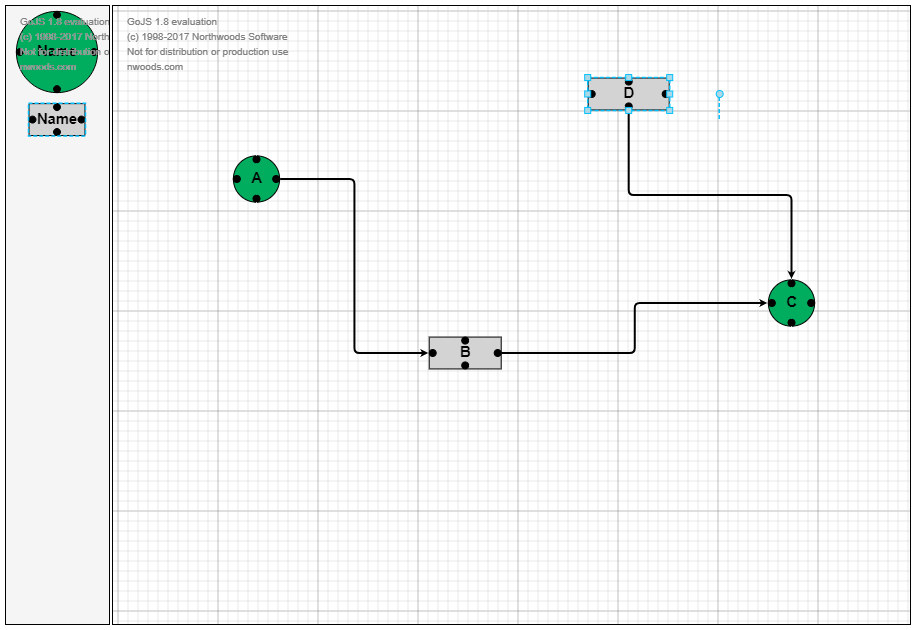
\includegraphics[scale=0.75]{gojssample.png}
	\caption{Ejemplo GoJS}\label{fig:gojssample}
\end{figure}

\vspace{5mm}

Para empezar, observando la figura anterior, cabe destacar que, para poder llevar a cabo este diagrama, es necesario reservar dos secciones del html (div). Una para la paleta de la izquierda contenedora de los elementos que son arrastrables, en este caso el círculo, y otro para el diagrama sobre el que se realizarán las acciones.


\vspace{5mm}

Para poder analizar detalladamente como se contruye a nivel Javascript la figura anterior, se irán explicando progresivamente los fragmentos del código que sean necesarios.

\vspace{5mm}

El elemento principal de esta estructura es el que contiene todo el resto y con el que posteriormente, en aplicaciones que integren el componente, se podrán comunicar, en este caso le llamaremos 'myDiagram'.

Lo principal de este diagrama es, como en todo lenguaje, darle un esqueleto, en GoJS los elementos adquieren dicha propiedad mediante la llamada a una librería de go llamada GraphObject bajo la sentencia make. Un ejemplo sencillo de creación de un diagrama sobre el espacio reservado del html llamado 'myDiagramDiv' es el siguiente:

\vspace{5mm}

\begin{figure}[H]
	\centering
	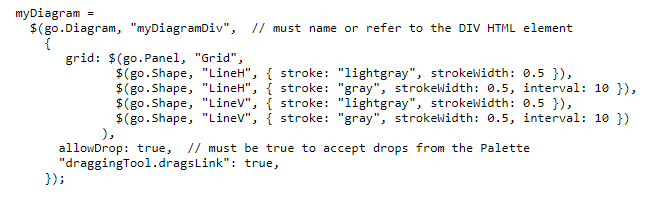
\includegraphics[scale=0.90]{creacionDiagramaGoJS.png}
	\caption{Creación Diagrama}\label{fig:creacionDiagramaGoJS}
\end{figure}

\vspace{5mm}
En la figura anterior se puede observar como se crea un diagrama. Además, se le asigna un grid o cuadrícula de fondo, así como, se le da la capacidad de poder arrastrar elementos sobre él.



\vspace{5mm}